\documentclass[a4paper, 11pt]{article}
\usepackage[italian]{babel}
\usepackage[utf8]{inputenc}
\usepackage{amsmath}
\usepackage{imakeidx}
\usepackage{amsfonts}
\usepackage{amssymb}
\usepackage{float}
\usepackage{graphicx}
\usepackage{caption}
\usepackage[paper=a4paper]{geometry}
\usepackage[shortlabels]{enumitem}
\usepackage{hyperref}
% Frontespizio config
\usepackage[nowrite]{front-th}
\usepackage{pdfpages}

\usepackage{fancyhdr} % <-- aggiunto
\pagestyle{fancy}     % <-- imposto lo stile fancy
\fancyhf{}
\rhead{\includegraphics[width=1cm]{Immagini/Logo_Università_di_Udine.png}} % <-- logo in alto a destra
\hypersetup{
    colorlinks,
    citecolor=black,
    filecolor=black,
    linkcolor=black,
    urlcolor=black
}

\setcounter{secnumdepth}{4}
\setcounter{tocdepth}{4}

% --- INIZIO SOSTITUZIONE MINTED CON LISTINGS ---
\usepackage{listings}
\usepackage{xcolor} % Necessario per definire i colori

\definecolor{codegray}{gray}{0.95}
\definecolor{codegreen}{rgb}{0.0, 0.5, 0.0} % Per i commenti
\definecolor{codered}{rgb}{0.9, 0.0, 0.0}   % Per le stringhe
\definecolor{codeblue}{rgb}{0.0, 0.0, 0.9}   % Per le parole chiave

\lstdefinestyle{mycodestyle}{
    backgroundcolor=\color{codegray}, % Colore di sfondo
    basicstyle=\small\ttfamily,       % Stile del testo del codice (dimensione piccola, font a spaziatura fissa)
    breaklines=true,                  % Permette al codice di andare a capo
    frame=single,                     % Aggiunge un bordo singolo
    framesep=5pt,                     % Spazio tra il bordo e il codice
    framerule=0.5pt,                  % Spessore del bordo
    rulecolor=\color{orange!70},     % Colore del bordo (arancione come nel tuo esempio)
    numbers=left,                     % Numerazione delle righe a sinistra
    numberstyle=\tiny\color{gray},    % Stile dei numeri di riga
    stepnumber=1,                     % Incremento dei numeri di riga
    numbersep=8pt,                    % Spazio tra numeri e codice
    showspaces=false,                 % Non mostrare spazi come simboli
    showtabs=false,                   % Non mostrare tab come simboli
    showstringspaces=false,           % Non mostrare spazi nelle stringhe
    commentstyle=\color{codegreen}\textit, % Stile per i commenti (verde, corsivo)
    keywordstyle=\color{codeblue}\bfseries, % Stile per le parole chiave (blu, grassetto)
    stringstyle=\color{codered},      % Stile per le stringhe (rosso)
    % Se vuoi un titolo/didascalia per il blocco di codice, potresti usare captionpos, ad esempio:
    % captionpos=b, % didascalia sotto
    % caption={Descrizione del codice},
}
% --- FINE SOSTITUZIONE MINTED CON LISTINGS ---


\renewcommand{\contentsname}{Indice}

\newcommand{\myfrontpage}{%
  \begin{titlepage}
  \centering
  \preparefrontpage
  \end{titlepage}
  \global\let\centering\relax % Disabilita centering globale
}

\fontoptionnormal

\makeatletter
\def\front@thecandidate{Candidato}
\def\front@thecandidates{Candidati}
\def\front@theadvisor{Relatore}
\def\front@theadvisors{Relatori}
\makeatother


% Dati frontespizio
\Universita{Udine}
\Logo[3.5cm]{./Immagini/Logo_Università_di_Udine.png}
\Dipartimento{Scienze Matematiche, Informatiche e Fisiche}  % Aggiunto in sostituzione di Facoltà
\Corso[Laurea]{Internet Of Things, Big Data, Machine Learning}
\Annoaccademico{2024--2025}
\Titolo{Laboratorio di Algoritmi e Strutture Dati\bigbreak - \bigbreak Verifica della complessità asintotica degli algoritmi di ordinamento}
\Candidato{Andrea Gioia - 169484}
\Candidato{Luca Gamberini - 168712}
\Relatore{Prof. Gabriele Puppis}
\Relatore{Prof. Carla Piazza}
% \Correlatore{Prof. Marco Sciandrone}  % Commentato come richiesto



\begin{document}
\myfrontpage

\thispagestyle{empty} 
%\preparefrontpage

\newpage

\tableofcontents
\newpage
\section{Introduzione}
Il progetto include le misurazioni e la conseguente graficazione di 4 algoritmi di ordinamento:
\begin{itemize}
    \item QuickSort
    \item QuickSort 3 Way
    \item CountingSort
\end{itemize}
\subsection{Specifiche tecniche}
Le specifiche tecniche delle misurazioni sono state:
\begin{itemize}
    \item Array generato con valori decimali \textbf{casuali}
    \item La lunghezza dell'array è compresa tra 100 e 100 mila valori
    \item Il valore di ciascun elemento dell'array varia casualmente tra 10 e un milione
\end{itemize}
Gli algoritmi sono stati implementati in linguaggio Python, mentre le misurazioni dei tempi sono state prese tramite la funzione \href{https://docs.python.org/3/library/time.html#time.perf_counter}{\textit{\texttt{perf\char`_counter}}} della libreria \textit{time}

\section{Algoritmi}
Gli algoritmi di ordinamento presi in esame presentano caratteristiche differenti e risultano più o meno efficienti in base alle carattestiche dell'array di elementi da ordinare.

\subsection{QuickSort}
Algoritmo di ordinamento ricorsivo del tipo divide-et-impera, quindi basato sulla suddivisione in n sottoproblemi, risolti ricorsivamente, fino al raggiungimento del caso base.\\
Non presenta la necessità di utilizzo di strutture dati aggiuntive, di conseguenza lo scambio di elementi avviene in-place.\bigbreak
Le complessità asintotiche temporali di QuickSort sono:
\begin{itemize}
    \item Caso ottimo: $\Omega(n\log_2n)$
    \item Caso medio: $\Theta(n\log_2n)$
    \item Caso pessimo: $\mathcal{O}(n^2)$
\end{itemize}

\subsubsection{Analisi delle complessità}
Il QuickSort è un esempio di algoritmo che lavora in-place, quindi la complessità in spazio equivale a $\Theta(n)$, ovvero la dimensione dell'array di partenza.\bigbreak
Le operazioni che influiscono sulla complessità di tempo sono:
\begin{itemize}
    \item Chiamata a partition, complessità $\Theta(n)$
    \item Le due chiamate ricorsive, complessità rispettivamente di $T(q-1)$ e $T(n-q)$.
\end{itemize}


L'equazione di ricorrenza di QuickSort è:
\begin{gather*}
    T(n) = 
    \begin{cases}
    \Theta(1)\quad\quad \text{se}\;\; n\; \leq\; 1 \\
    T(q - 1) + T(n - q) + \Theta(n)\quad\quad se\; n > 1
    \end{cases}     
\end{gather*}
 
\paragraph{Caso pessimo}\mbox{}\\
Nel caso pessimo, QuickSort ha complessità $\mathcal{O}(n^2)$.\\
La circostanza in cui QuickSort si trova nel caso pessimo è legata a una scelta sconveniente del pivot, il quale genera uno sbilanciamento nella divisione in parti dell'array.
\href{https://ifif.altervista.org/quicksort-come-funziona-esempio/?doing_wp_cron=1750427062.2481169700622558593750}{\color{blue}link alla fonte}.

\subsubsection{Codice}
\begin{lstlisting}[style=mycodestyle, language=Python]
def QuickSort( A, p, q ):
    if( p < q ):
        r = Partition( A, p, q)
        QuickSort( A, p, r-1 )
        QuickSort( A, r+1, q )
    return A

def Partition(A, p, q):
    x = A[q]
    i = p - 1
    for j in range(p, q):
        if A[j] <= x:   # (corretto A[j], non A[q])
            i += 1
            Scambia(A, i, j)
    Scambia(A, i + 1, q)    # posiziona il pivot al centro
    return i + 1

def Scambia(A, i, j):
    temp = A[i]
    A[i] = A[j]
    A[j] = temp
\end{lstlisting}
---Commento del codice---

\subsection{QuickSort3Way}
Versione modificata rispetto al QuickSort classico.\\
Prevede la suddivisione in 3 parti dell'array di elementi, sulla base di una variabile \textit{pivot}.\\
Gli scambi vengono fatti sulla base di un confronto tra elemento dell'array e la variabile pivot ($>$, $<$, $=$). Le chiamate ricorsive vengono effettuate su porzioni con elementi $<$ pivot e $>$ pivot.\\
A differenza del QuickSort classico, QuickSort3Way presenta notevole efficienza con array con molti elementi duplicati.\bigbreak
Le complessità asintotiche temporali di QuickSort3Way sono:
\begin{itemize}
    \item Caso ottimo: $\Omega(n\log n)$
    \item Caso medio: $\Theta(n\log n)$
    \item Caso pessimo: $\mathcal{O}(n^2)$
\end{itemize}

\subsubsection{Analisi delle complessità}
Come nel caso di QuickSort, anche il QuickSort3Way lavora in-place, senza bisogno di stutture dati aggiuntive, quindi la complessità in spazio è $\Theta(n)$.\\\\
Considerando che l'algoritmo itera gli elementi dell'array e siccome il ciclo for viene eseguito al massimo $n$ volte.\\
L'algoritmo partiziona l'array in tre sezioni (elementi $<$ pivot, $=$ pivot e $>$ pivot) attraverso un singolo passaggio che opera in tempo lineare $\Theta(n)$. La complessità temporale dipende dall'equilibrio delle partizioni:
\begin{itemize}
    \item \textbf{Caso ottimo ($\Omega(n \log n)$)}: Il caso ottimo si verifica quando il pivot divide in partizioni bilanciate l'array, di conseguenza in partizioni ciascuna di dimensioni $n/3$.
    \item \textbf{Caso medio ($\Theta(n \log n)$)}: La complessità resta invariata grazie alla gestione efficiente del confronto sugli elementi uguali, non andando a fare ulteriori confronti.
    \item \item \textbf{Caso pessimo ($\mathcal{O}(n^2)$)}: Occorre in situazioni in cui il pivot viene sistematicamente posizionato alla prima o all'ultima posizione dell'array. Questo va a creare partizioni sbilanciate. 
\end{itemize}


\subsubsection{Codice}
\begin{lstlisting}[style=mycodestyle, language=Python]
    def QuickSort3Way(arr, l, r):
    if l >= r:
        return

    lt = l
    i = l
    gt = r
    pivot = arr[l]

    while i <= gt:
        if arr[i] < pivot:
            arr[lt], arr[i] = arr[i], arr[lt]
            lt += 1
            i += 1
        elif arr[i] > pivot:
            arr[i], arr[gt] = arr[gt], arr[i]
            gt -= 1
        else:
            i += 1

    QuickSort3Way (arr, l, lt - 1)
    QuickSort3Way (arr, gt + 1, r)

    return lt, gt
\end{lstlisting}

\subsection{CountingSort}
CountingSort è un algoritmo di ordinamento non in-place, in quanto si avvale di un array aggiuntivo che conta il numero di occorrenze di ciascun elemento.\bigbreak
Le complessità asintotiche temporali di CountingSort sono:
\begin{itemize}
    \item Caso ottimo: $\Omega(n + k)$
    \item Caso medio: $\Theta(n + k)$
    \item Caso pessimo: $\mathcal{O}(n + k)$
\end{itemize}

\subsubsection{Analisi delle complessità}
CountingSort è un algoritmo stabile e senza confronto, il quale richiede la dichiarazione di un array ausiliario di dimensione \textit{max - min + 1}. Tutto ciò fa sì che la complessità in spazio di CountingSort sia $\mathcal{O}(n + k)$, dove $n$ è il numero di elementi dell'array e $k$ è pari all'ampiezza dell'intervallo di valori.\bigbreak
Essendo CountingSort un algoritmo di ordinamento senza confronto, il posizionamento degli elementi nell'array non influisce sulla sua efficienza, di conseguenza la complessità, sia nel caso ottimo, medio e pessimo, sarà sempre $\mathcal{O}(n + k)$; tuttavia, diventa inefficiente per intervalli di valori molto grandi ($k > n$). 


\subsubsection{Codice}
\begin{lstlisting}[style=mycodestyle, language=Python]
    def countingSort(arr):
    max = arr[0]
    min = arr[0]

    for i in range(1, len(arr)):
        if arr[i] > max:
            max = arr[i]
        elif arr[i] < min:
            min = arr[i]

    C = [0] * (max - min + 1)
    for i in range(len(arr)):
        C[arr[i] - min] += 1

    k = 0
    for i in range(len(C)):
        while C[i] > 0:
            arr[k] = i + min
            k += 1
            C[i] -= 1
\end{lstlisting}

\subsection{RadixSort}
RadixSort è un algoritmo di ordinamento basato sull'ordinamento cifra per cifra, partendo da quella meno significativa. Risulta particolarmente efficiente in presenta di molti numero con la stessa quantità di cifre.\bigbreak
Le complessità asintotiche temporali di RadixSort sono:
\begin{itemize}
    \item Caso ottimo: $\Omega(n\cdot d)$
    \item Caso medio: $\Theta(n\cdot d)$
    \item Caso pessimo: $\mathcal{O}(n\cdot d)$
\end{itemize}

\subsubsection{Motivazioni della scelta}
É stato scelto RadixSort come quarto algoritmo a scelta per il suo approccio innovativo e diverso rispetto agli altri algoritmi selezionati, offrendo una prospettiva di confronto interessante.

\subsubsection{Analisi delle complessità}
L'algoritmo RadixSort richiede due array ausiliari, uno di dimensione pari alla base numerica scelta, e l'altro di dimensione n (numero di elementi). Di conseguenza, la complessità in spazio dell'algoritmo è pari a $\mathcal{O}(n + b)$.\bigbreak
Nel caso ottimo, tutti gli elementi hanno lo stesso numero di cifre. Considerando $d$ come il numero delle cifre, la complessità totale sarà $\mathcal{O}(d(n + b))$.\bigbreak
Nel caso pessimo, tutti gli elementi hanno lo stesso numero di cifre, ad eccezione di un elemento che avrà un numero di cifre molto più elevato. Se il numero di cifre dell'elemento più grande è pari a $d$, la complessità temporale diventa $\mathcal{O}(d (n + b))$. Mediamente, la complessità temporale nel caso medio di RadixSort è di $\mathcal{O}(d (n + b))$, dove $n$ è il numero di elementi e $b$ è la base di rappresentazione.

\subsubsection{Codice}
\begin{lstlisting}[style=mycodestyle, language=Python]
def RadixSort(arr):
    radix_array = [[], [], [], [], [], [], [], [], [], []]  # array delle cifre
    max_val = max(arr)  # assegno il valore massimo dell'array
    exp = 1 

    while (max_val // exp) > 0:
        while len(arr) > 0:
            val = arr.pop()
            radix_index = (val // exp) % 10
            radix_array[radix_index].append(val)

        for bucket in radix_array:
            while len(bucket) > 0:
                val = bucket.pop()
                arr.append(val)

        exp *= 10
\end{lstlisting}

\section{Misurazioni}

\begin{table} [H]
    \centering
    \begin{tabular}{|c|c|}
        \hline
        QuickSort \\ [0.1 cm]
        \hline
    \end{tabular}
\end{table}

\begin{figure} [H]
    \centering
    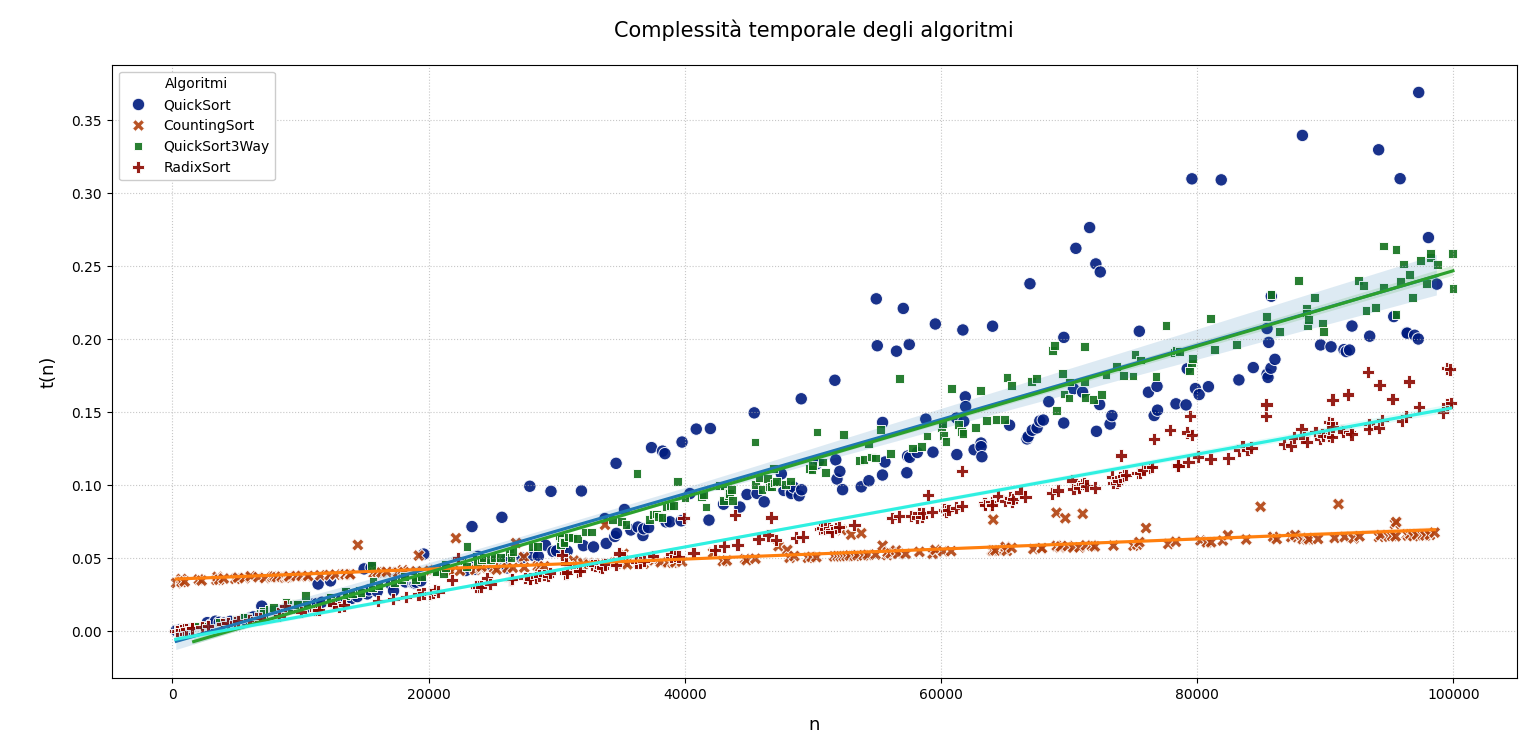
\includegraphics[scale=0.5]{Immagini/Grafico.png}
    \caption*{Parte reale sulle x, parte immaginaria sulle y}
\end{figure}

\section{Conclusione}
Conclusione della relazione.

\end{document}